\documentclass{standalone}
\usepackage{amsmath,amssymb,amsthm}
\usepackage{tikz}
\usetikzlibrary{decorations.markings}
\usetikzlibrary{arrows,automata}
\usetikzlibrary{positioning}
\usetikzlibrary{arrows.meta,positioning}

\begin{document}
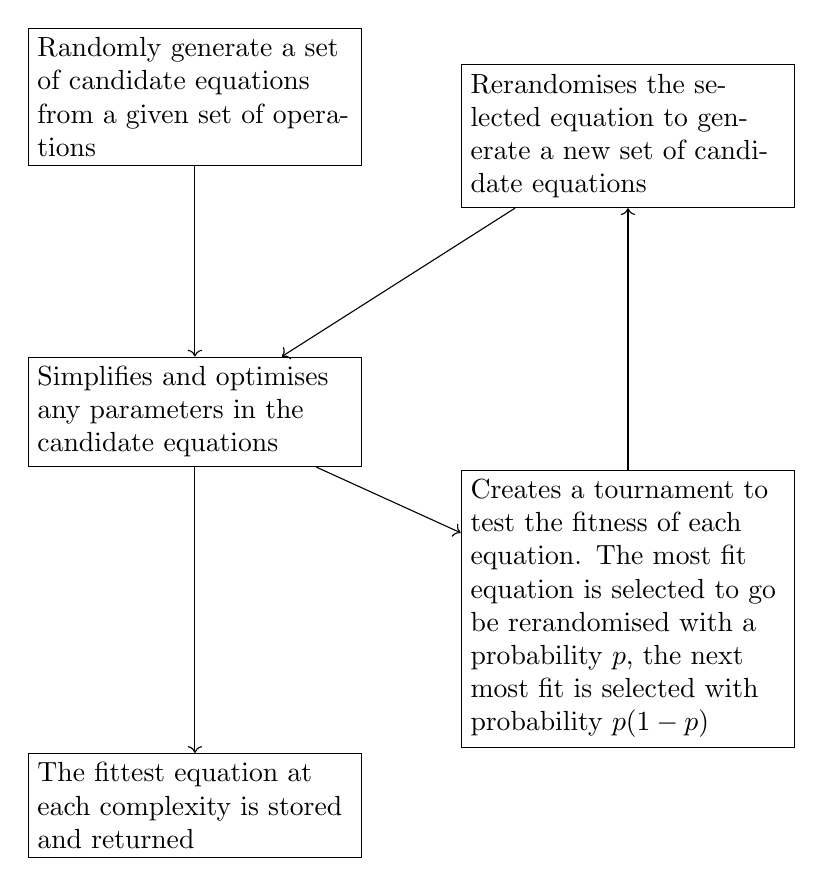
\begin{tikzpicture}[
    mycircle/.style={
        circle,
        draw=black,
        fill=black,
        fill opacity = 1,
        inner sep=0pt,
        minimum size=5pt,
        font=\small},
    nocircle/.style={
        circle,
        draw=black,
        fill=black,
        fill opacity = 1,
        inner sep=0pt,
        minimum size=0.45pt,
        font=\small},
    targetcircle/.style={
        circle,
        draw=red,
        fill=red,
        fill opacity = 1,
        inner sep=0pt,
        minimum size=5pt,
        font=\small},
    myarrow/.style={->},
    dottedarrow/.style={-,dashed},
    thicccarrow/.style={->,line width=5pt},
    node distance=1.2cm and 1.5cm
]


\begin{scope}
    \begin{scope}
        \node[draw,text width=4cm] (a) at (0,0) {Randomly generate a set of candidate equations from a given set of operations};

        \node[draw,text width=4cm] (b) at (0,-4) {Simplifies and optimises any parameters in the candidate equations};

        \node[draw,text width=4cm] (c) at (5.5,-6.5) {Creates a tournament to test the fitness of each equation. The most fit equation is selected to go be rerandomised with a probability $p$, the next most fit is selected with probability $p(1-p)$};

        \node[draw,text width=4cm] (d) at (5.5,-0.5) {Rerandomises the selected equation to generate a new set of candidate equations};

        \node[draw,text width=4cm] (e) at (0,-9) {The fittest equation at each complexity is stored and returned};
    \end{scope}


    \path[every node/.style={font=\sffamily\small}] 
        (a) edge[myarrow] [color=black] (b)
        (b) edge[myarrow] [color=black] (c)
        (d) edge[myarrow] [color=black] (b)
        (c) edge[myarrow] [color=black] (d)
        (b) edge[myarrow] [color=black] (e);
\end{scope}
\end{tikzpicture}
\end{document}